%%%%%%%%%%%%%%%%%%%%%%%%%%%%%%%%%%%%%%%%%%%%%%%%%%%%%%%%%%%%%%%%%%%%%%%%%%%%
\vspace{-4mm}
\section{Scientific Motivation}
\label{sec:motivation}
\vspace{-3mm} 

The universe is magnetized on nearly every scale -- magnetic fields
can be seen in the intergalactic and interstellar medium, in
molecular clouds, and in stars.  The universe also appears to be
magnetized over a wide range of cosmic time, with evidence for
magnetic fields observed at high redshift as well as in the local
universe.  Magnetic fields are dynamically important in many of the
observed astrophysical environments, having energy densities that are
comparable to (or in equipartition with) other available energy
sources, including heat, turbulence, cosmic rays, and radiation.
Furthermore, even in situations where magnetic fields are dynamically
irrelevant (such as the intergalactic plasma in clusters of galaxies),
they are critical for processes such as thermal conduction and particle
acceleration.  Magnetic fields (and dust pinned to them) also give rise to the
majority of the polarized microwave sky, which is an important contaminant for
studies of the cosmic microwave background.  

%In some extremely diffuse plasmas, magnetic
%fields are the only mechanism that causes particles to behave as a
%fluid!  In addition, magnetic fields are a useful probe of
%astrophysical plasma physics, but are often challenging to use as an
%observational diagnostic due to fundamental uncertainties in
%measurements (e.g., the need to assume a coherence length to interpret
%Faraday rotation measure observations).

%In the following sections, we describe what is known about magnetic
%fields in the universe, both observationally and theoretically, and
%highlight some of our gaps in understanding.  \textbf{In general, while
%magnetic fields have been measured in virtually all astrophysical
%regimes, and while there is a clear sequence of events -- galaxies
%form molecular clouds, which in turn are the sites of star formation
%-- the ways in which magnetic fields tie galaxies to molecular clouds,
%and thus potentially affect star formation and the stellar initial
%mass function, are poorly understood theoretically.}
 
\vspace{-3mm}
\subsection{The high-redshift universe}
\label{sec:extragalactic}
\vspace{-2mm}

There is evidence that magnetic fields have existed
over much of the age of the universe.  Observations of high-redshift
quasar absorption line spectra show that MgII absorption lines are
associated with large Faraday rotation measures, requiring that
organized magnetic fields of strengths comparable to those observed in
galaxies today ($\sim \mu$G) must have existed by $z \approx 1.3$,
less than half of the age of the universe \cite{2008Natur.454..302B, Joshi13,
Farnes14}.  In related observations, \cite{2008ApJ...676...70K} use
observations of rotation measures in a large sample of quasars that
extends to $z \simeq 3.7$ to show that the distribution of rotation
measures broadens with redshift (despite the expected cosmological
`dilution' of high redshift rotation measures expected by the
expanding universe), and that at increasing redshift progressively
fewer sources are found with small rotation measures in the observer
frame.  The implications of this observation are that the environments
of high-redshift ($z \sim 2-3$) galaxies were significantly
magnetized, with the possibility that magnetic field strengths in
galaxies at this epoch -- a few billion years after the Big Bang --
are comparable to those seen in present-day galaxies.  
%This work
%broadly agrees with earlier observations of $z \sim 2-3$ radio
%galaxies \cite{1998A&A...329..809A}, which showed different
%rotation measures between the two radio lobes of the observed
%galaxies.  The most obvious interpretation of this difference is
%that it comes from the radio galaxy itself, and the inferred magnetic
%fields have strengths on the order of a few $\mu$G.

Beyond statistically detecting magnetic fields in high redshift
galaxies, major progress has been made in mapping magnetic fields in
individual cosmologically-distant galaxies. Recently, 
\citet{Mao17} have exploited the scenario where a background
polarized source was lensed by a foreground galaxy at $z=0.439$ to
detect an axisymmetric microgauss magnetic field in the lensing galaxy
as seen $\sim 4.6$ billion years ago.  This is the highest redshift
galaxy for which we have both magnetic field strength and structure
information, and which can be used to test dynamo theories.  In
particular, this paper puts a clear upper limit of a few Gyr on the
timescale for creating strong, coherent magnetic fields in galaxies!

% The
% authors of that work are currently extending this work to others
% gravitationally-lensed galaxies to provide even stronger constraints
% on the growth of large-scale galactic magnetic fields as a function of
% redshift.

%
In addition to existing in galaxies over a wide span of time, the
presence of magnetic fields has been inferred on cosmological scales
in the intergalactic medium.  At megaparsec scales,
\cite{2010Sci...328...73N} show that the lack of measured GeV
gamma-rays in the direction of TeV gamma-ray sources observed by the
Fermi Large Area Telescope yields a \textit{lower bound} of B~$\geq 3
\times 10^{-16}$~G, with the lower bound increasing as $\propto
\lambda_B^{-1/2}$ if the magnetic field correlation length $\lambda_B$
is significantly smaller than a megaparsec.  Different analyses of
data from the same instrument by \cite{2011ApJ...733L..21D,
2010MNRAS.406L..70T}, with varied assumptions, results in lower limits
for the strength of large-scale magnetic fields in the low redshift
intergalactic medium that range from $\geq 10^{-18}$ G to $\geq 5
\times 10^{-15}$~G.  None of these observations provides direct
measurements of the coherence lengths of the fields in question,
though they are inferred to be on the order of megaparsecs or greater.
Also, it should be noted that these are lower limits on the large-scale intergalactic
magnetic field and not a direct measurement.  An upper limit can also be determined by using the
cosmic microwave background (CMB) -- specifically, measurements of CMB
temperature anisotropies and polarization put strong upper limits on a
mean pre-recombination magnetic field strength $\simeq 10^{-9}$~G
\cite{1997PhRvL..78.3610B,2012SSRv..166...37W,2013A&ARv..21...62D}.
We note that the CMB-derived
upper limit is more stringent than the limits
coming from Big Bang Nucleosynthesis, where measurements of the ratios
of primordial species (including H, D, and He), as well as the
baryon-to-photon ration $\eta$, give a strong upper limit for
primordial magnetic field strengths of $10^{-7}$~G.

Intergalactic magnetic fields on smaller scales have also been
observed.  Rotation measure observations of the intracluster medium
-- that is, the intergalactic plasma in clusters of galaxies -- show
that it is threaded by magnetic fields that are on the order of
$0.1-10$~$\mu$G (depending on cluster location)
\cite{Carilli02,2005mpge.conf..231E, 2005A&A...434...67V}, with
patches of much higher magnetization ($\sim 40$~$\mu$G) observed.
Furthermore, ``cool core'' clusters tend to have stronger fields by a
factor of roughly 2 than non-cool core clusters.  The same
observations show that magnetic fields are not regularly ordered on
cluster scales, but instead have coherence lengths that range from a
few kpc to tens of kpc. It is very difficult to discern the volume
filling fraction of magnetic fields in the intracluster medium due to
the paucity of background sources that can be used to observe rotation
measures -- however, essentially all background sources show some
magnetization.


\vspace{-3mm}
\subsection{Low-redshift galaxies}
\label{sec:lowz}
\vspace{-2mm}

% note: can use \begin{wrapfigure}{R}{0.65\textwidth} if we really want.
%\begin{figure}[t]


Observations of magnetic fields in nearby galaxies provide an
important complement to measurements of magnetic fields in both the
intergalactic medium and at high redshift.  Recent work by Van Eck
et al. \cite{2014arXiv1411.1386V} consolidates data on the properties
of the magnetic fields and interstellar media of 20 local spiral
galaxies, and \citet{Tabatabaei16} find that magnetic field scales with galaxy
mass.
%, with selected results shown in
%Figure~\ref{fig:bfield_spirals}.  
All galaxies have detectable
magnetic fields with ordered field strengths on the order of $1-10$~$\mu$G, and
total field strengths roughly 5 times larger, $5-50$~$\mu$G, which is
roughly in equipartition with the cosmic ray and kinetic energy
densities (a result that has been confirmed elsewhere; \cite{Mao12,
Beck13}), and which are coherent on large scales.  Clear correlations
exist between the total magnetic field strength and molecular gas
density, as well as the star formation rate.  Furthermore, the
magnetic pitch angle correlates well with the mean axisymmetric
magnetic field strength, but not with the local rotational shear rate.
\citet{2014arXiv1411.1386V} also compare their results with predictions from galactic
dynamo theory, and note that while some of the observations agree with
these predictions, there is clear need for further theoretical work.
Separately, observations of M33 (a nearby face-on spiral galaxy) show
that the magnetic fields in six giant molecular cloud complexes are
aligned with the spiral arms, which strongly suggests that the
large-scale field in M33 anchors the molecular clouds
\citep{2011Natur.479..499L}.  Results such as this one will provide
strong constraints on simulations that model the relationship between
molecular clouds and the galaxies that contain them. 

%\begin{wrapfigure}{l}{0.5\textwidth}

M
%\begin{center}
%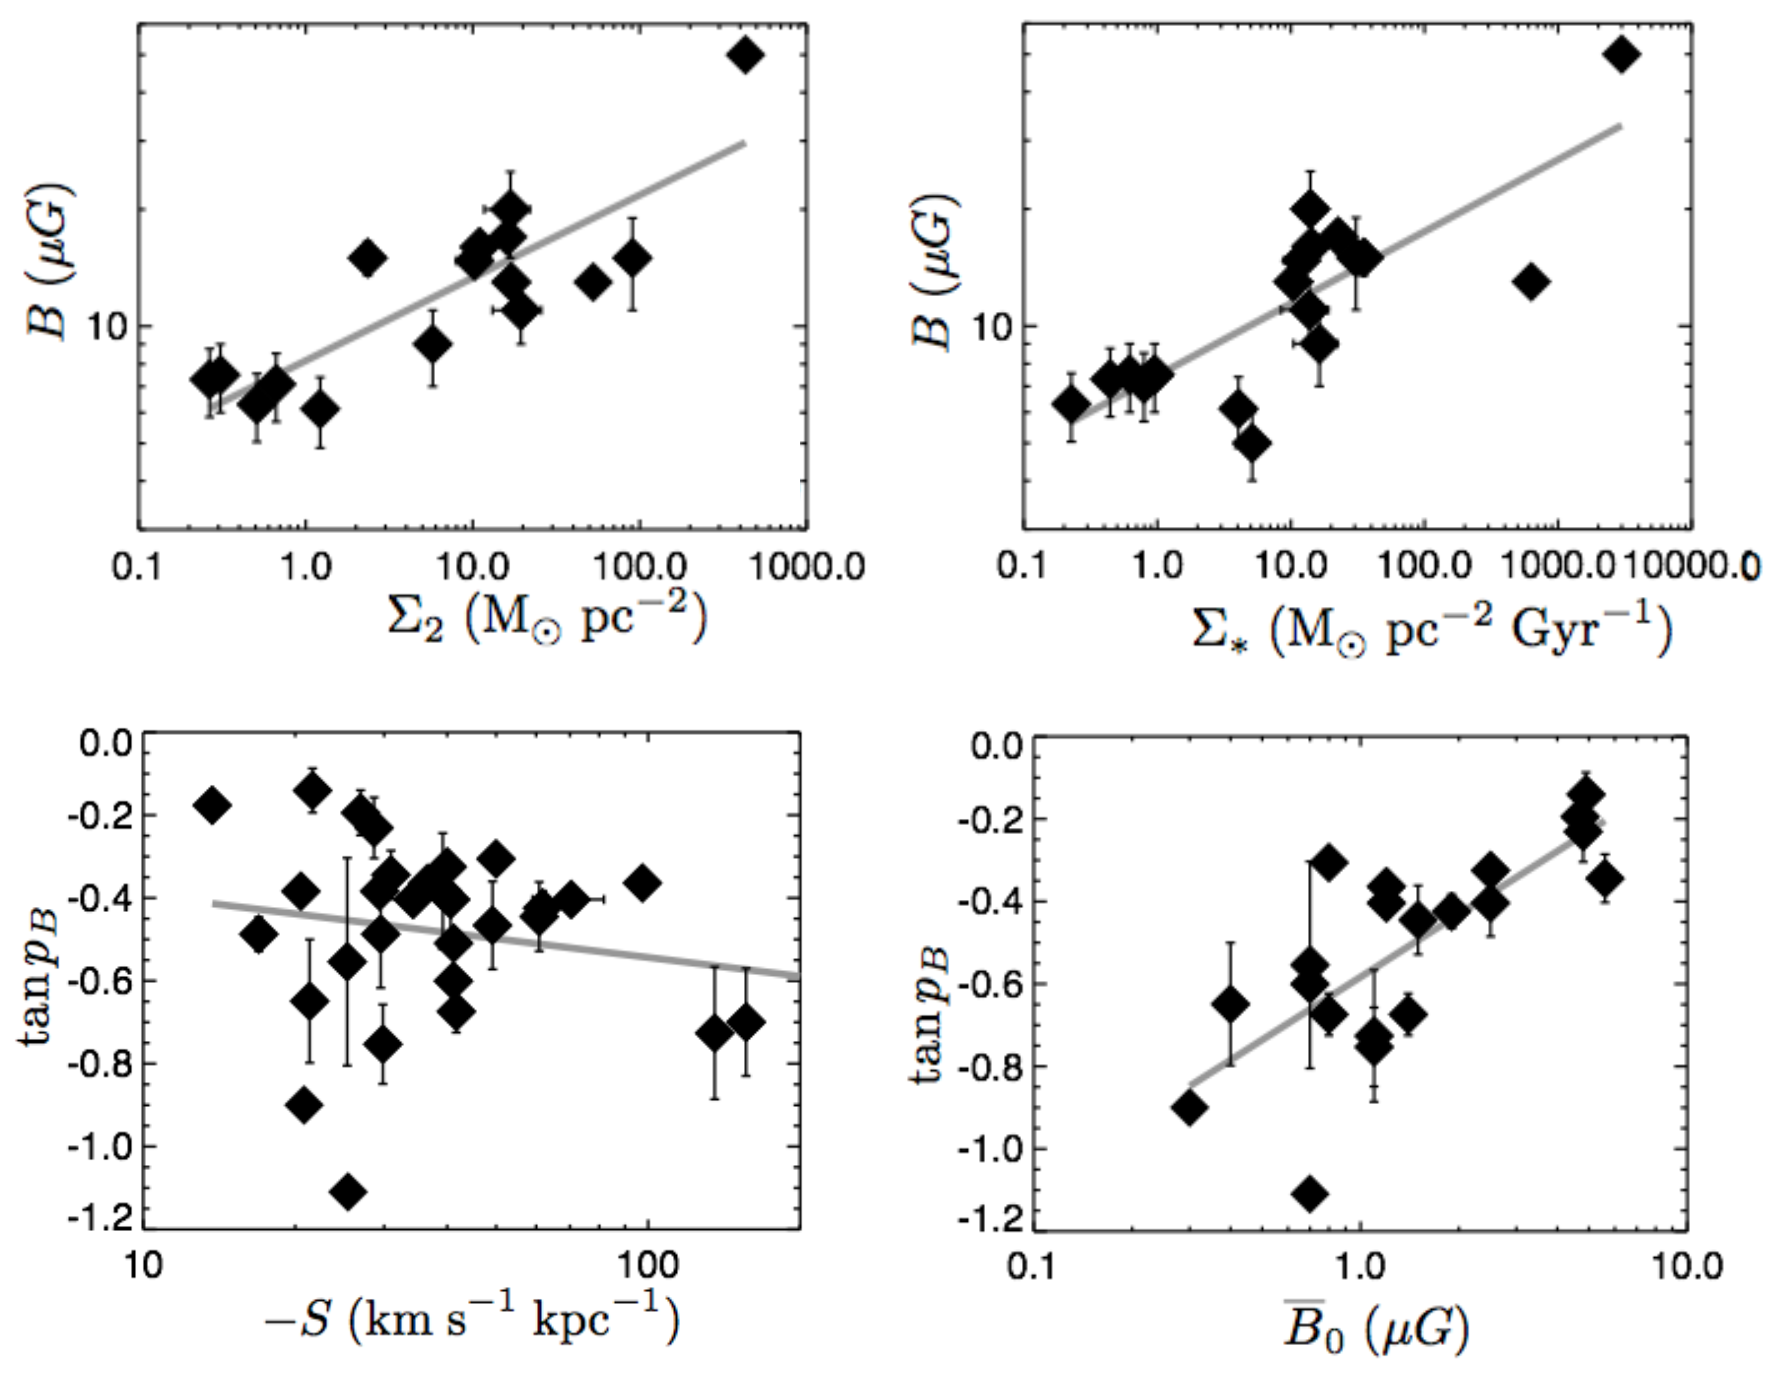
\includegraphics[width=0.48\textwidth]{VanEck.png}
%\end{center}
%\vspace{-6mm}
%\caption{\label{fig:bfield_spirals} 
%  Magnetic field properties from a sample of 20 nearby spiral galaxies
%from Van Eck et al. \cite[][panels taken from Figures 4 and 9]{2014arXiv1411.1386V}.  Top row: Total
%magnetic field strength vs. H$_2$ surface density (left) and vs. star
%formation rate surface density (right).  Bottom row: Pitch angle of
%mean magnetic field vs. rotational shear rate (left) and
%vs. axisymmetric component of the large-scale magnetic field (right).
%While \cite{2014arXiv1411.1386V} find close correlations between a
%variety of properties, not all are easily explicable via galactic dynamo
%theory.}
%\vspace{-3mm}
%\end{wrapfigure}
Measurements of magnetic field properties in other types of local
galaxies have been made as well.  Field strengths in local elliptical
galaxies are believed to be on the order of $5-10$~$\mu$G, comparable to local
spirals, although with much smaller coherence lengths -- far smaller
than the size of the galaxy itself
\cite{1993A&ARv...4..449W,1996MNRAS.279..229M}, though to date no conclusive
measurement has been made.  Field strengths in
dwarf galaxies have been measured to have total 
strengths ranging from $5-15$~$\mu$G and ordered fields having strengths
of $1-8$~$\mu$G, generally a few times weaker than local spirals,
depending on the galaxy in question
\cite{2000A&A...355..128C,2011A&A...529A..94C,2012MNRAS.423L.127R,Mao12,2013MNRAS.435..149N,2014A&A...567A.134J}.
We do note that dwarf galaxies with lower masses do tend to have lower
total and ordered magnetic field strengths than larger dwarfs
and spirals, and galaxies with higher star formation rates also
tend to have higher magnetic field strengths (as was seen in spirals
in \cite{2014arXiv1411.1386V}).  Furthermore, it seems that, for dwarf
galaxies where the structure of the magnetic field strength can be
measured, the ordered component is about $20\%$ as strong as the total
magnetic field, which is comparable to much more massive local spiral galaxies.

\vspace{-3mm}
\subsection{The Milky Way}
\label{sec:milkyway}
\vspace{-2mm}

The best candidate for obfuscating the picture of magnetic fields in galaxies is
our own Milky Way.  The proximity to the source means that high resolution
measurements can be made, but our location within the galactic disk means that comparing
to other galaxies is difficult.  Faraday rotation and polarization of other
galaxies measures the field strength integrated through the entire thickness of
the disk, while similar measurements of our own galaxy only sample fractions of
the field.  Further, many local radio features (such as the north
polar spur and other magnetized loops and filaments) make it difficult
to disentangle larger-scale magnetic field structures.

The magnetic field in the Milky Way's disk can be broken into two
components: a large scale magnetic field that has a coherence length
on the order of the size of the Galaxy itself, and a small scale field
that is either completely random or somewhat correlated with the large
scale field.  Synchrotron radio emission indicates that the large
scale field strength is roughly 10 $\mu$G at a Galactocentric radius
of 3 kpc, and decreases to 6 $\mu$G near the Sun.  This is consistent
with Zeeman measurements of nearby molecular clouds (see Section
\ref{sec:conngalmcs}).  Estimates of the strength of the random
magnetic field component varies from $B_{\rm{rand}} \gtrsim
1.3$~$\mu\rm{G}$ \citep{Gaensler01} to $4$~$\mu\rm{G}$
\citep{Fauvet11}.
The most complete survey of dust polarization was performed by the
\emph{Planck} satellite \citep{PlanckIntermediateXIX15}, which can be seen in
the right panel of Figure \ref{fig:bfield_morphology}.  Clearly structure can
be seen on a range of scales throughout the galactic disk.

The morphology of the magnetic field in external spirals is generally parallel
to spiral arms, as shown in the left panel of Figure \ref{fig:bfield_morphology}.  This is
likely the case with the Milky Way.  However, unlike other galaxies, the Milky Way
seems to additionally harbor at least one reversal in the direction of the
magnetic field
\citep{Thomson80, Jaffe11}.  Many models exist to match the data \citep[see the
recent review by][]{2015ASSL..407..483H}, including an antisymmetric spiral (similar to
other galaxies), a bisymmetric spiral (which would account for reversals), a
ring structure, and some superposition of these.  The vertical component of the
Galactic magnetic field is similarly difficult to measure.  Using rotation
measure from more than 1,000 extragalactic radio sources, \cite{Mao10} find
that there is no symmetry in the vertical component at the radius of the sun,
with the Galactic north field showing a field consistent with zero, and the
Galactic south field of $0.31 \pm 0.03 \mu$G.  On the other hand,
\cite{Jansson12} find that, modeling the synchrotron intensity from WMAP, the
field is consistent with an ``X'' shaped magnetic field.
Unfortunately, none of the existing measurements are 
consistent with expected observations and a coherent dynamo. This is
possibly due to the fact that the timescale for the coherent $\alpha-\Omega$
dynamo is longer than the age of the Galaxy, or if tidal interactions or
injection of small scale magnetic fields continually disrupt the symmetry
\citep{Moss12}.  

Another potentially important reservoir of  magnetic field energy is in the Milky Way's
circumgalactic medium (CGM), which is the huge volume of hot, diffuse
baryons that exists outside of the stellar disk but within the virial
radius of the dark matter halo.  The CGM  contains approximately half
of the baryons in the entire Milky Way system \citep[see,
e.g.,][]{2014ApJ...786...54P}, and is considered to be important for
the regulation of the star formation history of galaxies, and also responsible for
controlling the bulk scaling relations  seen in local galaxies
\citep{2015ApJ...808L..30V,2017ApJ...845...80V}.  The CGM is
metal-enriched, and thus is likely to be
substantially magnetized assuming that both metals and magnetic fields
originate in stars.  Some evidence exists for large-scale
magnetic fields in the CGM \citep[see,
e.g., Figure 7 in][]{2017ARA&A..55..111H}, but the detailed structure
of the circumgalactic magnetic will require the Square Kilometer Array
or one of its pathfinders as a probe \citep{2015aska.confE..41H}.

One of the primary motivations for this study is the spatial distribution and
correlations in the magnetic field, and the synchrotron and polarized dust
emission that is dictated by these correlations.  These are important
foregrounds for studies of the polarized cosmic microwave background (CMB), and
and understanding the location and structures the magnetic field produces is
essential for their removal.  These signals occupy different
locations in the galaxy, with the polarized dust emission at relatively low
galactic scale height and the synchrotron coming from higher, hotter gas.  
The polarized signal is best observed by converting it to two rotationally
invariant quantities, $E$ and $B$.  The former is parity-even, while the latter
is parity-odd \citep{Seljak97,Seljak97b,Kamionkowski97}. The spectral
amplitudes, $C_\ell^{EE}$ and $C_\ell^{BB}$ have been found 
that these amplitudes scale as a powerlaw in the wavenumber, $\ell^\alpha$ where
$\alpha=-2.4$, and has roughly twice the power in $E$ than $B$ \citep{Planck2016,Planck2018}.  This is
intriguingly smooth over the high-latitude sky.  Preliminary studies of both
galactic magnetic field \citep{Kim19} and driven turbulence \citep{Kritsuk19}
 have shown promising reproduction of this signal.  The proposed work will complement these works by
examining the impact of the formation history and circumgalactic environment on
the spatial distribution and structures in the polarized gas.  

The statistical separation of the ISM and CMB signals is a necessary component
of their removal.
This is subject of a separate
proposal that we are submitting, and beyond the scope of this one.  This
proposal seeks to understand the components of the signal, and provide maps for
training of cleaning algorithms. 


\begin{figure}[t]
\begin{center}
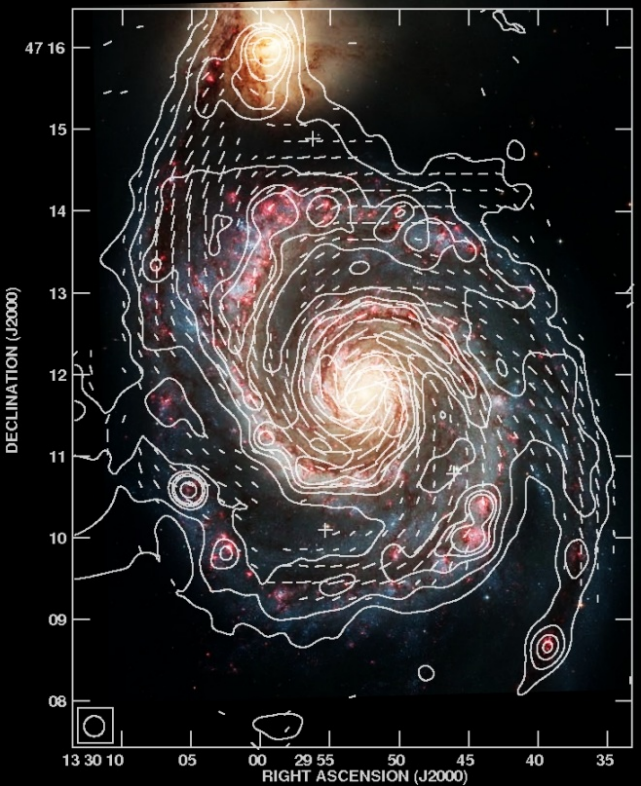
\includegraphics[width=0.29\textwidth]{Fletcher.png}
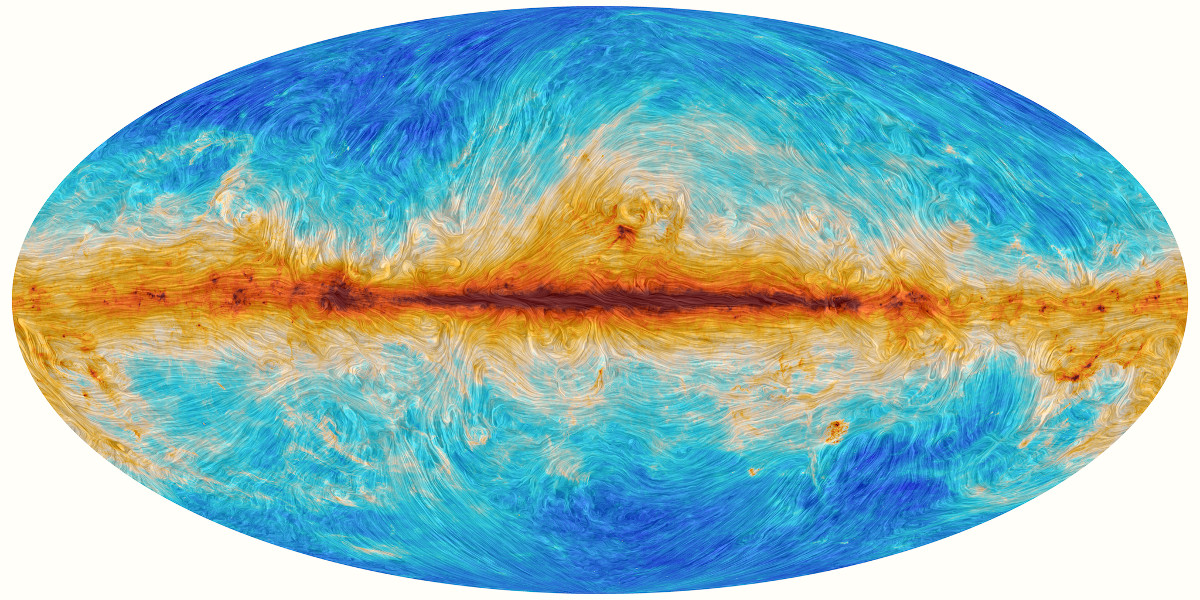
\includegraphics[width=0.69\textwidth]{Planck.jpg}
\end{center}
\vspace{-6mm}
\caption{\label{fig:bfield_morphology} Coherent magnetic structure is seen in
many disk galaxies. (\emph{Left}) The magnetic field from
polarized $\lambda=3,6$ and 20 cm  radio emission (vectors) along with total
emission (contours) in M51. From  \cite{Fletcher11}.  Optical background from \emph{Hubble Space Telescope}
(image credit: NASA, ESA, S. Beckwith (STScI) and The Hubble Heritage Team
(STScI/AURA)).  This shows the well-ordered nature of the magnetic field along
the spiral arms. 
(\emph{Right}) The \emph{Planck} polarization map showing the 353 GHz dust
intensity convolved with the direction of polarization
\citep{PlanckIntermediateXIX15}.  This shows coherent structrue on a range of
scales throughtout the Milky Way.
%(\emph{Right})  From \cite{Noutsos12}, the inferred magnetic
%field direction in the Galaxy (green vectors) as compared to spiral arms (white
%boxes).  Measurements from rotation measure from 622 pulsars, with field
%direction towards the sun in blue, red away from the sun.  Clearly reversals in
%the mean field are seen in the Galaxy, but not in M51
}
\vspace{-3mm}
\end{figure}

\vspace{-2mm}
\subsection{Connecting galaxies to molecular clouds}
\label{sec:conngalmcs}
\vspace{-2mm}

%This impacts our
%understanding of cloud formation as well as cloud lifetime and collapse, and,
%ultimately, star formation rates, masses, and binary rates.  Clearly there is
%order on the tens of kpc scale (e.g. Figure \ref{fig:bfield_morphology} from
%\citet{Fletcher11}), which is much larger than the 1-100 pc scale of molecular
%clouds.   
%The galactic magnetic field also has small-scale fluctuations
%\citep{2015ASSL..407..483H}, which is unsurprising as the ISM is also clearly 
%turbulent.  Simulations of multiphase magnetized ISM result in molecular gas with
%weak magnetic fields \citep{deAvillez05, Kritsuk09c}, while observations are
%ambiguous, 


Molecular Clouds and Giant Molecular Clouds are cold (10 K) and have masses
anywhere from $10^4-10^7$~M$_\odot$.  From the limited number of Zeeman splitting measurements in cold molecular
clouds, field strengths in molecular clouds range from 1 $\mu$G in low
density  gas ($\simeq 100$ \percc), and increase to a few mG in higher density gas
($\simeq 10^7$ \percc) \citep{Crutcher12}.  Star formation is controlled by some
combination of gravity, turbulence, and magnetic fields \citep{McKee07}, and 
the relative
importance of each is the subject of significant debate \citep[compare, e.g.,][]{Padoan13,
Li14}.   
The ratio of
magnetic to kinetic energy is typically parameterized by the \alf\ Mach number,
$\alfmach=v/v_{\rm{A}}$, where $v_{\rm{A}} = B/4 \pi \sqrt{\rho}$ is the signal
speed along a magnetic field line.  Values of $\alfmach>1$, so-called \sa\
flow, indicates a weak magnetic field relative to kinetic energy, while
$\alfmach<1$, or \suba\ flow, indicates that magnetic fields dominate energetically.  The ratio of
gravitational to magnetic energy is typically parameterized by the mass-to-flux
ratio, $\mu=M/\Phi$, where $\Phi$ is the magnetic flux threading a cloud of mass
$M$, in units of the critical field strength for collapse.  The actual values of
$\alfmach$ and $\mu$ are difficult to
measure observationally due to the challenge in measuring magnetic
field strengths directly over large scales
\citep{Crutcher12}. 
 Thus, statistical and morphological arguments are made,
often with different results.   From measurements of column density power
spectra and extinction measure distribution in molecular clouds,
\cite{Padoan99} and \cite{Padoan04c} argue that \sa\ turbulence is more
consistent with molecular cloud measurements than the statistics of \suba\
models.  On the other hand, \cite{Heyer12} have shown that a difference in the
slope of the velocity power spectrum between two orthogonal directions indicates that
$\alfmach\approx 1$.  Simulations \citep{deAvillez05, Kritsuk11c}
 indicate that
$\alfmach>1$ for clouds that formed from the warm neutral medium. 
Polarization
measurements indicate that fields are parallel to the long axis of low mass
filaments, 
perpendicular to the long axis of high mass filaments \citep{Li13}, and exhibit coherent
alignment between large and small scales \citep{Li09}, all of which indicate
$\alfmach<1$.
Zeeman measurements of methanol masers in star forming
region indicate that the
magnetic field order is imprinted on even small-scale structures over kpc
scales.
\citep{Green12}.  
However,
 turbulence substantially impacts the
structure of molecular clouds \citep[see, e.g.,][]{Elmegreen04, MacLow04}, and statistical
properties indicate that turbulent kinetic energy is comparable to, if not dominant over,
magnetic energy \citep{Padoan04, Heyer12}, indicating $\alfmach\gtrsim 1$.
Figure \ref{fig:SFR} shows the connection between molecular clouds and magnetic
fields, in the left panel, in observations of field alignment with spiral
structure, from \citet{2011Natur.479..499L}, and the connection between field
and the halo in a pilot study for the proposed work.

 The details of the initial conditions, boundary conditions, and
equation of state have profound impact on molecular cloud lifetimes and collapse rates
\citep{Federrath12, Collins12, Rey-Raposo14}.
Furthermore, even in
models of star-forming clouds where magnetic fields play a subordinate role their
effect is still non-negligible.  
Thus it is clear that for a
detailed understanding of star formation, magnetic fields must be included.
In order to capture these conditions self-consistently, \textbf{we will
perform extremely high resolution simulations of
isolated galaxies, extracted from cosmological initial conditions, that resolve the formation of a wide mass range of
molecular clouds.} 

%\dcc I cut this text.
%Magnetic fields can aid in the
%formation of molecular clouds by way of magnetic instabilities such as the
%Parker instability \citep{Parker66}, wherein buoyant, magnetized clouds of gas
%lose mass preferentially along magnetic fields into magnetic valleys, possibly
%%coalescing gas into massive structures \citep{Kim03}.  Alternatively, magnetic
%fields lend support against self-gravitating disk instabilities \citep{Kim01}
%and Jeans instabilities \citep{Elmegreen87}. 



\begin{figure}[t]
\begin{center}
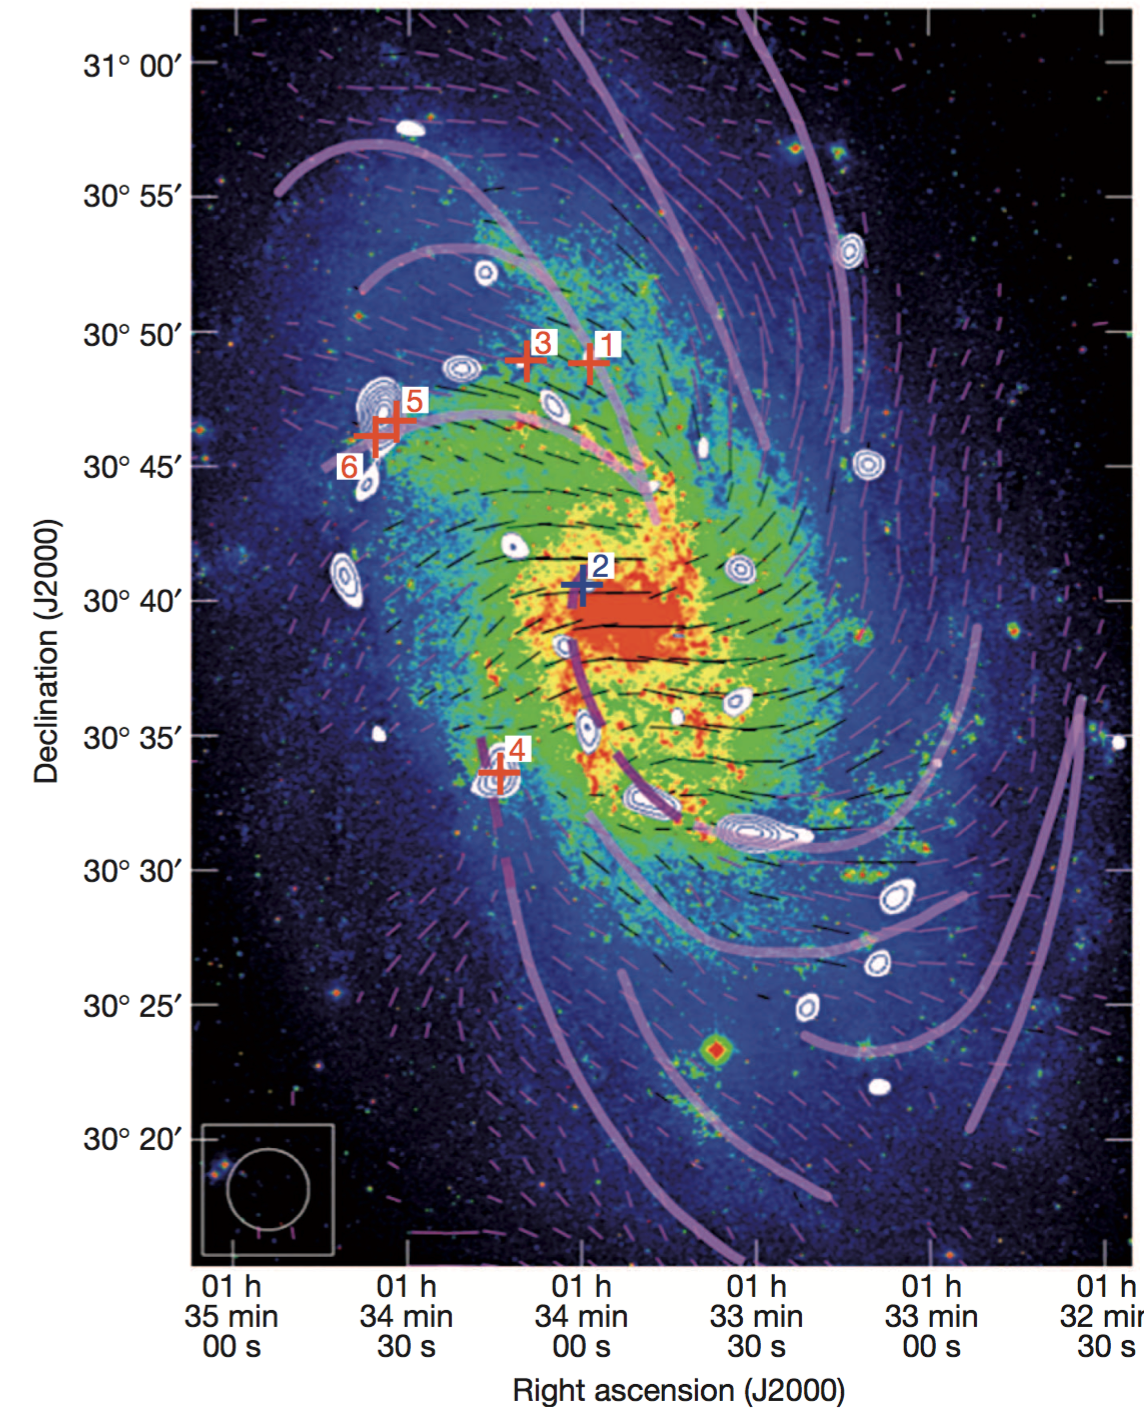
\includegraphics[width=0.23\textwidth]{LiHenning.png}
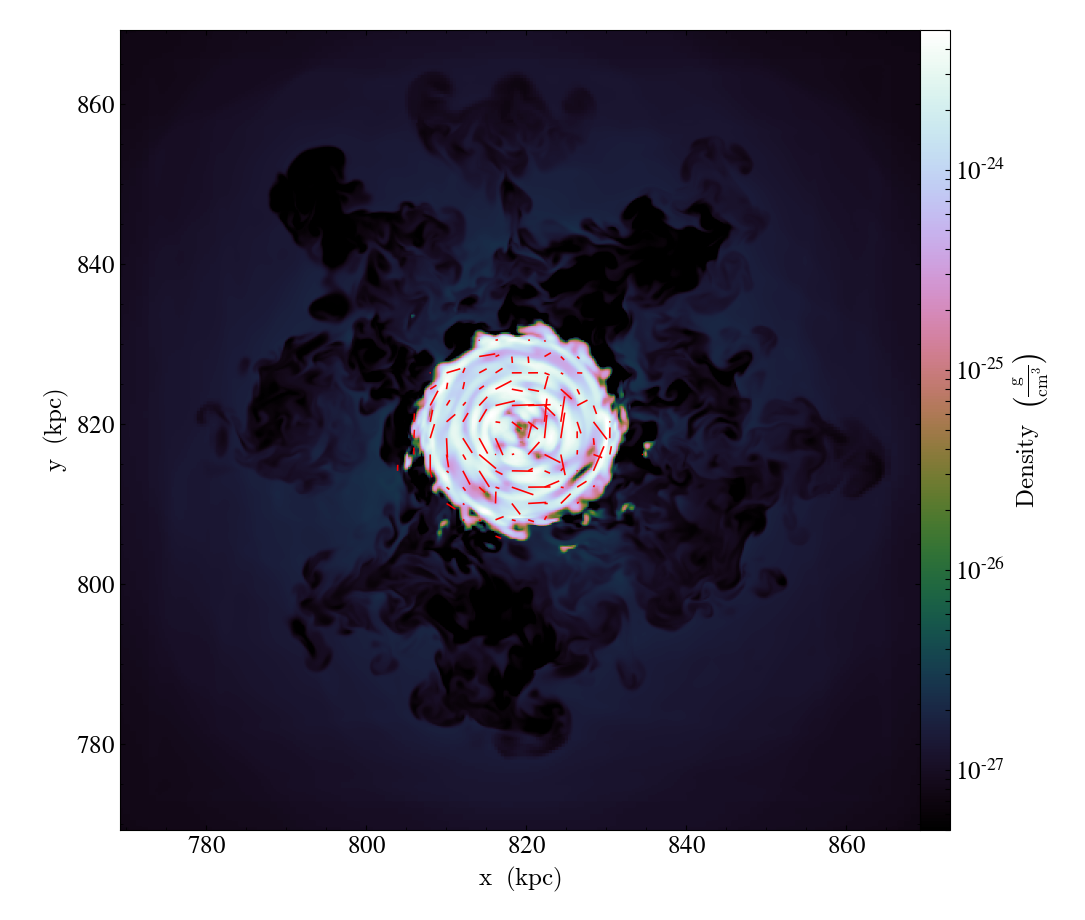
\includegraphics[width=0.346\textwidth]{g30_g18d_annotate_7.png}
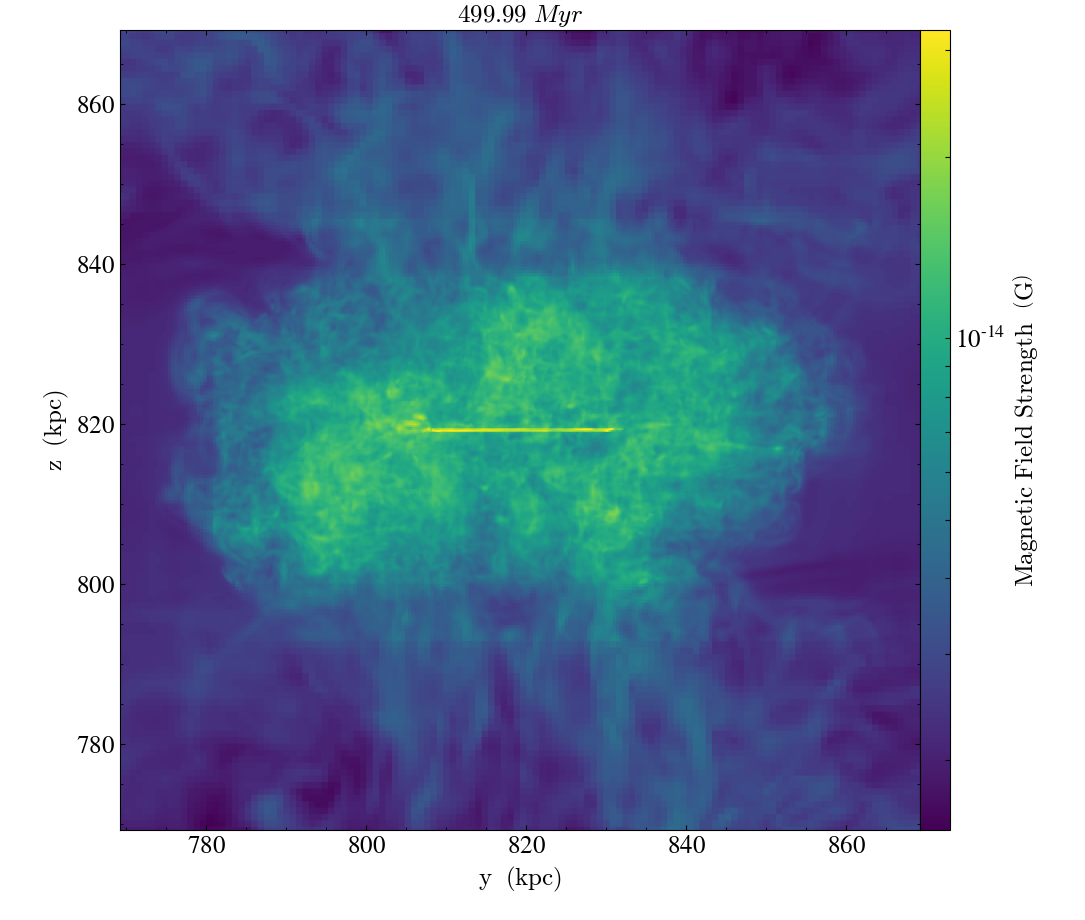
\includegraphics[width=0.346\textwidth]{g18d_0100_Projection_x_magnetic_field_strength_ones.png}
\end{center}
\vspace{-6mm}
\caption{\label{fig:SFR}
\emph{(Left)}: From \citet{2011Natur.479..499L}, magnetic fields in molecular
gas (thin lines) traces spiral arms (thick lines) in M33.
\emph{(Center, Right)} 
From preliminary galaxy-scale simulations with an initial
uniform field of $10^{-15}\rm{G}$ a Milky Way sized galaxy 
produces fields up to $10^{-13}\rm{G}$ at 20 kpc from the disk within 500 Myr.  
The center panel shows synthetic polarization direction following the rotational
structure.  The right panel shows mean magnetic field strength in an edge-on
projection.
This simulation has an
under-resolved ISM in the galaxy, and serves as a pilot study for the proposed
work. }
\vspace{-3mm}
\end{figure}

\vspace{-3mm}
\subsection{The origin and amplification of magnetic fields in the universe}
\label{sec:origins}
\vspace{-2mm}

% \brian Where do magnetic fields come from in the Universe?  Not 100\%
% clear yet.  High-z magnetogenesis; Biermann battery during structure
% formation and in stars; outflows.  In galaxies, mostly from
% stars/supernovae and amplification of existing b-fields due to the
% dynamo process.  Sum up MHD simulations of cosmological structure
% formation!

As discussed in Section~\ref{sec:extragalactic}, magnetic fields
appear to exist everywhere in the intergalactic medium, albeit at a
very low level.  The physical regimes where they appear to reside --
on megaparsec scales and above, and in both intergalactic filaments
and in voids -- argue against a galactic origin.  So, then, what is
the likely origin of these fields, and what theoretical constraints
can we utilize?

Widrow \cite{2002RvMP...74..775W,2012SSRv..166...37W} provides a host
of possible origins for the observed cosmological magnetic fields,
which we briefly summarize.  Magnetic fields could be generated during
the inflationary epoch, during the hadronic or electroweak phase
transitions, or in the radiation-dominated era prior to recombination.
Depending on the nature of the effect, theoretical predictions for a
minimum field strength vary hugely, from a minimum value of B~$\sim
10^{-32}$~G to substantially more than a Gauss (values given at the
present day).  Generally speaking, theory dictates that a minimum
magnetic field strength of $10^{-19}$~G (present-day value) and with
coherence lengths on megaparsec scales must exist; the maximum
theoretically-predicted value is vastly higher than the observational
upper limits from the CMB of $\bar{B} \simeq 10^{-9}$~G (Section~\ref{sec:extragalactic}).

Given the minuscule magnetic field strengths that must have been
generated prior to structure formation, and the relatively high ($>
10$~$\mu$G) fields observed in both galaxies and the cores of galaxy
clusters, an obvious question arises: how are such high magnetic
fields generated from such weak seed fields?  Straightforward
adiabatic collapse of the gas (and corresponding compression of the
fields) suggests an increase in magnetic field from the initial value
of $\delta^{2/3}$, where $\delta$ is the ratio of maximum to original
density.  Given the characteristic density of the Milky Way's
interstellar medium, this implies an adiabatic amplification of
$\simeq 10^4 - 10^5$ times the primordial value -- far too small of a
value to explain the roughly 13 order of magnitude difference between
the minimum inferred value in the lowest-density regions of the
universe and the field strength observed in the interstellar medium.

This observation leads inexorably to the conclusion that there must be
some sort of dynamo process at work that amplifies the magnetic field
by using kinetic energy from the various processes associated with
structure formation (i.e., gravitational collapse, rotational motion,
etc.).  There are two dominant modes of amplification.  The
\emph{fluctuating} dynamo draws small scale turbulent energy into
small scale magnetic energy.  While this mechanism has growth times of
$10^7$ years (fast enough to generate substantial fields from
extremely weak seed fields), it does not produce fields that are
ordered on large scales.  The second amplification mechanism is the
$\alpha-\Omega$ dynamo, wherein differential rotation and buoyancy
work together to add helicity to the fluid, thus amplifying the field
on the large scales associated with the rotation of the galaxy.  This
is a slower process, which limits the large scale field available to
more massive galaxies.  (See \cite{Brandenburg05} for a detailed
review of both dynamo processes.)  Either of these processes can
easily magnify a seed field to the galactic field
strength of $10^{-6}$~G \cite{Beck13}, and compression by
gravitational collapse further amplifies the galactic field strength
and is responsible for the further magnification of the field to the
$10^{-3}$~G level observed in high-density star forming regions
\cite{Collins11}.  We note that further seeds beyond the weak
primordial field may be necessary to reach the observed magnetic field
strengths in galaxies, particularly for the earliest galaxies --
observations of strong magnetic fields at high redshift imply that
dynamos have a relatively short time to operate!  If that is the case,
two plausible mechanisms for initial magnetic field generation are supernova
remnants \cite{2002RvMP...74..775W} and the jets from supermassive
black holes \cite{1969Natur.223..936H, 1990ApJ...364..451D}, both of
which produce strong magnetic fields with substantial coherence
lengths.

